\hypertarget{problems}{%
\section{Problems}\label{problems}}

\begin{enumerate}
\item
  What is the difference between \emph{effect} and \emph{affect}?
\item
  Why is simulation useful to roboticists?
\item
  List some of the advantages and disadvantages of simulating a robot
  vs. working with physical robots.
\item
  Assume that you have a two link manipulator with \(a_1 = 15\)cm and
  \(a_2 = 15\)cm and that the base of the manipulator is at the origin
  of the coordinate system. Write a Python program to take the list of
  workspace points and plug them into the inverse kinematics formulas
  for the two link manipulator. Plot these points on a graph where
  \(\theta_1\) is the horizontal axis and \(\theta_2\) is the vertical
  axis. You will have to adjust some aspects to get a good looking plot.
  (Scale factors etc.) Test your code on the workspace line

  (a) \(x+y = 25\), \(x, y >0\) and (b) \(x = 10\cos (t) + 15\),
  \(y = 10\sin (t)\) for \(0 \leq t \leq \pi\). The point here is to see
  what the configuration space curve looks like.
\item
  Assume that you have a two link manipulator with \(a_1 = 15\)cm and
  \(a_2 = 15\)cm and that the base of the manipulator is at the origin
  of the coordinate system. Write a two link manipulator location
  program (Python). This program will take a list of angles and compute
  the location of the end effector. Show how this program works with the
  list of angles you generated in the previous problem. If the angle
  inputs are generated by a square, the simulated robot arm's end
  effector should trace a square. Plot the end effector points. You need
  to plot the input shape and the final shape to see if your code is
  correct. You will need to use the previous problem for this problem.
  Demonstrate your code to trace out the four segments which form the
  square with endpoints (5,0), (5, 15), (20, 15), (20,0).
\item
  Assume that you have a parallel two link manipulator with
  \(L_0 = 10\)cm, \(L_1 = 15\)cm and \(L_2 = 20\)cm. Write a Python
  program to take the list of workspace points given and plug them into
  the inverse kinematics formulas for the two link manipulator. Plot
  these points on a graph where \(\theta_1\) is the horizontal axis and
  \(\theta_2\) is the vertical axis. As above, you will have to adjust
  some aspects to get a good looking plot. The point here is to see what
  the configuration space curve looks like. The workspace points are the
  list of points for the rectangle with corners (-5, 18), (5, 18), (5,
  27), (-5,27). Use 10 points in each side of the rectangle.
\item
  Assume that you have a parallel two link manipulator with
  \(L_0 = 10\)cm, \(L_1 = 15\)cm and \(L_2 = 20\)cm. Write a Python
  program that will take a list of angles and compute the location of
  the end effector. Show how this program works with the list of angles
  you generated in the previous problem. {[}If the angle inputs are
  generated by a rectangle, the simulated robot arm's end effector
  should trace a rectangle.{]} Plot the end effector points. You will
  need to use the previous problem for this problem.
\item
  Using Numpy and the linspace command, build an array of points for
  \texttt{Fig:shapeforhw}. The top is given by
  \((x-10)^2 + (y-8)^2 = 25\) and the bottom is the line segment along
  \(y=8\). Traverse the figure starting at the right corner, going
  counter clockwise (circle first) and ending on the line segment. Check
  this with the Python plot command. Show the result.

  \leavevmode\hypertarget{Fig:shapeforhw}{}%
  \begin{figure}
  \centering
  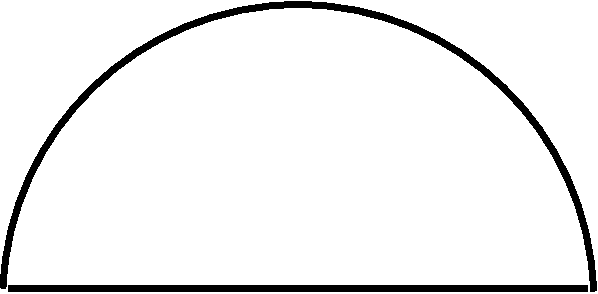
\includegraphics[width=0.35\textwidth,height=\textheight]{SimulationFigures/halfcircle.*}
  \caption{Half disk.}
  \end{figure}
\item
  Using Python and ZeroMQ, write a chat program (call it
  \emph{chat.py}). First prompt the user for their name. Write to all
  members in the chat group that this person has entered the chat. In a
  loop, grab user inputs and broadcast to the chat with format: name:
  \textless user input\textgreater{} . Echo to the terminal all strings
  sent to the chat.
\item
  Using Python and ZeroMQ, modify the example programs in the text on
  the kinematics of the two link manipulator.

  \begin{enumerate}
  \tightlist
  \item
    Write a program that creates a list of 100 equally spaced points
    along the path \(y = 15 -  x\) for \(0 \leq x \leq 10\) and
    publishes those points on the topic {physData} using a multiarray
    floating data type, i.e. values x and y are floats. Publish the data
    at 5Hz.
  \item
    Write a program that subscribes to topic {physData}, plugs the
    values in, computes the serial two link inverse kinematics to gain
    the servo angles (pick one of the +/-) and publishes the angles to
    the topic /thetaData. You may assume the link arms are
    \(a_1=a_2 = 10\). Format will be the same as the previous topic.
  \item
    Write a program that subscribes to both {physData} and {thetaData}.
    The program should plug the angles into the forward kinematics and
    check against the data in {physData}. It should plot the original
    curve in green and the ``check'' in blue.
  \end{enumerate}
\item
  Assume that you have a parallel two link manipulator with
  \(L_0 = 10\)cm, \(L_1 = 15\)cm and \(L_2 = 20\)cm.

  \begin{enumerate}
  \tightlist
  \item
    Write a ZeroMQ program that creates a list of 100 equally spaced
    points along the path \(x = 7\cos(t)+10\), \(y = 5\sin(t) + 15\) and
    publishes those points on the topic {physData} using a multiarray
    floating data type, i.e. values x and y are floats. Publish the data
    at 5Hz.
  \item
    Write a ZeroMQ program that subscribes to topic {physData}, plugs
    the values in, computes the serial two link inverse kinematics to
    gain the servo angles and publishes the angles to the topic
    {thetaData}. Format will be the same as the previous topic.
  \item
    Write a ZeroMQ program that subscribes to both {physData} and
    {thetaData}. The program should plug the angles into the forward
    kinematics and check against the data in {physData}. It should plot
    the original curve in green and the ``check'' in blue.
  \end{enumerate}
\item
  Using Python and 0MQ write a program that will add padding to
  obstacles while shrinking the footprint of the robot to a point.
  Assume that you have a circular robot with radius 10 and starting pose
  (15,15,90).

  \begin{enumerate}
  \tightlist
  \item
    Write a program that will publish the pose of the robot on the topic
    {robot\_pose} and the footprint type of the robot on
    {robot\_footprint} as a string (For example circle or polygon). Also
    publish the radius of the robot on {robot\_radius}.
  \item
    Write a program that will publish a list of obstacles as polygons on
    the topic {obstacles}. For this program let the obstacles be the
    following:

    \begin{enumerate}
    \tightlist
    \item
      Rectangle with the vertices (40,30), (50,5), (50, 30) (40,30).
    \item
      Rectangle with the vertices (40,5), (50,5), (50,0), (40,5).
    \end{enumerate}
  \item
    Write a program that subscribes to {robot\_pose},
    {robot\_footprint}, and {obstacles}. Based on the footprint string,
    this program should be able to subscribe to either the robot radius
    or dimension topics for circular and rectangular robots. This
    program will reduce the robot footprint to a point, add padding to
    the obstacles, and plot the robot as a point and padded obstacles
    with the maximum x and y values being 70 and 30.
  \end{enumerate}
\item
  Rework the previous problem assuming that you have a rectangular robot
  with \(width=10\) and \(length=20\) and initial pose (0,10,0).
\item
  Using Python and ZeroMQ, write a program to calculate the motion of a
  differential drive robot.

  \begin{enumerate}
  \def\labelenumii{\alph{enumii}.}
  \tightlist
  \item
    Write a program that publishes a sequence of wheel velocities on the
    topic {WheelVel} at 10Hz. Use the multiarray datatype. This node
    should be named {Control}. This program should also publish on a
    topic named {Active} either 1 or 0 at 1 Hz to say whether or not the
    robot is active (meaning done with wheel velocities and you can plot
    now: active =1, done = 0). Demonstrate the code on
    \(\dot{\phi}_1 = 2 + 2e^{-t_n}\) and \(\dot{\phi}_2 = 2+e^{-2t_n}\)
    for \(0 \leq t \leq 10\).
  \item
    Write a program that uses the differential drive kinematics to
    derive the robot linear and angular velocities. Publish the
    velocities using a message and name the topic {RobotVel}. This node
    should be named {ForwardK}. Assume that \(D=10\), \(L=20\) and the
    robot starts at (0,0,0).
  \item
    Write a program that will subscribe to the message and plot the
    robot's path using Python plotting when it gets the signal on the
    Active topic. This node should be named {RobotPlot}.
  \end{enumerate}
\item
  Using the above problem, replace the initial pose (0,0,0) in the
  second part, (b), with the pose (2,2,45).
\item
  Using the forward difference on \(x(t) = t^2\), what is the error on
  the derivative value for
  \(\Delta t  = 10^{-1}, 10^{-2}, 10^{-3}, 10^{-4}\) at the location
  \(t=1\).
\item
  Let \(r=10\), \(L=20\), \(\Delta t = .1\). Find the discrete kinematic
  model if the wheel velocities are \(\dot{\phi}_{1} = 2(1-e^{-t})\),
  \(\dot{\phi}_{2} = 2(1-e^{-2t})\).
\item
  Using the discrete model equations in the previous, plot the path for
  \(0 \leq t \leq 5\).
\item
  For the integral in \texttt{ddexamplenotworkable}, use a numerical
  differential equation solver (with some software package) to integrate
  the equations. Compare this to using a Taylor expansion on the
  equations to work out the integrals.
\item
  What is the smooth (\(\dot{x}\), \(\dot{y}\) are continuous)
  parametric form of

  \begin{enumerate}
  \def\labelenumii{\alph{enumii}.}
  \tightlist
  \item
    \(y=(3/2)x + 5/2\)
  \item
    \(y = x^{2/3}\).
  \item
    \((x-3)^2/16 + (y-2)^2/9 = 1\).
  \end{enumerate}
\item
  Find the analytic wheel velocities and initial pose for a differential
  drive robot tasked to follow (\(r=1\), \(L=4\)) the given paths. Plot
  the paths and compare to the actual functions to verify.

  \begin{enumerate}
  \def\labelenumii{\alph{enumii}.}
  \tightlist
  \item
    \(y=(3/2)x + 5/2\)
  \item
    \(y = x^{2/3}\)
  \item
    \((x-3)^2/16 + (y-2)^2/9 = 1\)
  \end{enumerate}
\item
  Find the wheel velocities and initial pose for a differential drive
  robot tasked to drive a square with corners (0,0), (10,0), (10,10),
  (0,10). You should stop and turn at a corner. Drive the edges at unit
  speed. Plot the paths and compare to the actual functions to verify.
\item
  Find the wheel velocities and initial pose for a differential drive
  robot in an infinity (\(\infty\)) shape. Plot the paths and compare to
  the actual functions to verify.
\item
  Write robot control code to drive the robot along the indicated paths
  and plot the obstacles and paths in matplotlib.

  \begin{enumerate}
  \def\labelenumii{\alph{enumii}.}
  \tightlist
  \item
    the triangular path with vertices (0,0), (15,0) , (5,20),
  \item
    the square path with corners (0,0), (10,0), (10,10), (0,10),
  \item
    the circular path centered at the origin and radius is 15.
  \end{enumerate}
\item
  Create two circular obstacles. The first obstacle is a disk centered
  at (5,5) with radius 2. The second is a disk centered at (15,15) with
  radius 3. Write the control code to drive a figure 8 around the two
  obstacles. Run at least two loops. Plot the obstacles and path in
  matplotlib.
\end{enumerate}
